\documentclass[a4paper]{article}

\usepackage{amsmath,amsthm,amssymb}
\usepackage{tikz}
\usetikzlibrary{arrows}
\usetikzlibrary{external}
\tikzexternalize[prefix=figures/]

\tikzset{
every node/.style={circle, draw, inner sep=2pt},
every label/.style={rectangle, draw=none}
}

\begin{document}

%%%%%%%%%%%%%%%%%%%%%%%%%%%%%%%%%%%%%%%%%%%%%%%%%%
\verb|shortestAB|

\tikzsetnextfilename{shortestAB}
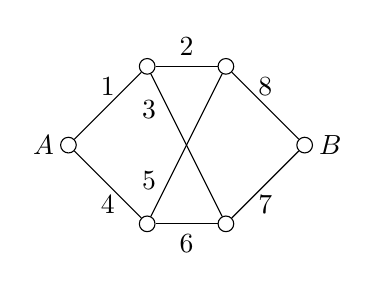
\begin{tikzpicture}
\node[label={left:$A$}] (0)  at (0,0) {};
\node (1)  at (1,1) {};
\node (2)  at (1,-1) {};
\node (3)  at (2,1) {};
\node (4)  at (2,-1) {};
\node[label={right:$B$}] (5)  at (3,0) {};

\draw (0) --node[midway,above,draw=none] {$1$} (1);
\draw (0) --node[midway,below,draw=none] {$4$} (2);
\draw (1) --node[midway,above,draw=none] {$2$} (3);
\draw (1) --node[near start,left,draw=none] {$3$} (4);
\draw (2) --node[near start,left,draw=none] {$5$} (3);
\draw (2) --node[midway,below,draw=none] {$6$} (4);
\draw (3) --node[midway,above,draw=none] {$8$} (5);
\draw (4) --node[midway,below,draw=none] {$7$} (5);
\end{tikzpicture}


%%%%%%%%%%%%%%%%%%%%%%%%%%%%%%%%%%%%%%%%%%%%%%%%%%
\verb|tickets-directed|

\tikzsetnextfilename{tickets-directed}
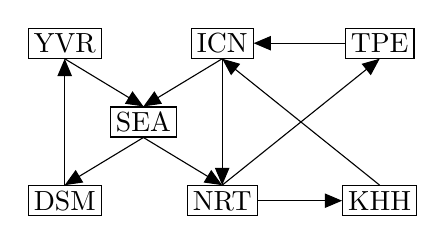
\begin{tikzpicture}
\node [rectangle] (YVR) at (-1,1) {YVR};
\node [rectangle] (DSM) at (-1,-1) {DSM};
\node [rectangle] (SEA) at (0,0) {SEA};
\node [rectangle] (ICN) at (1,1) {ICN};
\node [rectangle] (NRT) at (1,-1) {NRT};
\node [rectangle] (TPE) at (3,1) {TPE};
\node [rectangle] (KHH) at (3,-1) {KHH};

\draw[-triangle 45] (YVR.south) -- (SEA.north);
\draw[-triangle 45] (SEA.south) -- (NRT.north);
\draw[-triangle 45] (NRT.east) -- (KHH.west);
\draw[-triangle 45] (KHH.north) -- (ICN.south);
\draw[-triangle 45] (ICN.south) -- (NRT.north);
\draw[-triangle 45] (NRT.north) -- (TPE.south);
\draw[-triangle 45] (TPE.west) -- (ICN.east);
\draw[-triangle 45] (ICN.south) -- (SEA.north);
\draw[-triangle 45] (SEA.south) -- (DSM.north);
\draw[-triangle 45] (DSM.north) -- (YVR.south);
\end{tikzpicture}


%%%%%%%%%%%%%%%%%%%%%%%%%%%%%%%%%%%%%%%%%%%%%%%%%%
\verb|tickets-directed-imp|

\tikzsetnextfilename{tickets-directed-imp}
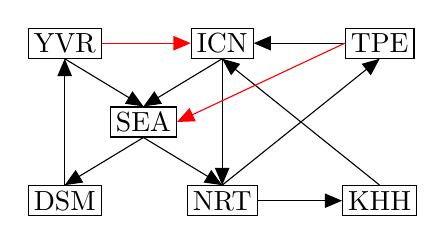
\begin{tikzpicture}
\node [rectangle] (YVR) at (-1,1) {YVR};
\node [rectangle] (DSM) at (-1,-1) {DSM};
\node [rectangle] (SEA) at (0,0) {SEA};
\node [rectangle] (ICN) at (1,1) {ICN};
\node [rectangle] (NRT) at (1,-1) {NRT};
\node [rectangle] (TPE) at (3,1) {TPE};
\node [rectangle] (KHH) at (3,-1) {KHH};

\draw[-triangle 45] (YVR.south) -- (SEA.north);
\draw[-triangle 45] (SEA.south) -- (NRT.north);
\draw[-triangle 45] (NRT.east) -- (KHH.west);
\draw[-triangle 45] (KHH.north) -- (ICN.south);
\draw[-triangle 45] (ICN.south) -- (NRT.north);
\draw[-triangle 45] (NRT.north) -- (TPE.south);
\draw[-triangle 45] (TPE.west) -- (ICN.east);
\draw[-triangle 45] (ICN.south) -- (SEA.north);
\draw[-triangle 45] (SEA.south) -- (DSM.north);
\draw[-triangle 45] (DSM.north) -- (YVR.south);
\draw[-triangle 45,red] (TPE.west) -- (SEA.east);
\draw[-triangle 45,red] (YVR.east) -- (ICN.west);
\end{tikzpicture}


%%%%%%%%%%%%%%%%%%%%%%%%%%%%%%%%%%%%%%%%%%%%%%%%%%
\verb|tickets-simple|

\tikzsetnextfilename{tickets-simple}
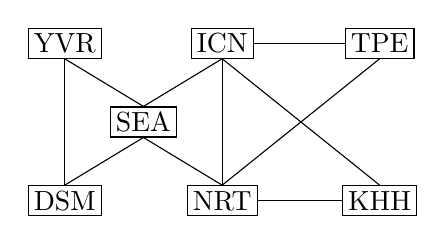
\begin{tikzpicture}
\node [rectangle] (YVR) at (-1,1) {YVR};
\node [rectangle] (DSM) at (-1,-1) {DSM};
\node [rectangle] (SEA) at (0,0) {SEA};
\node [rectangle] (ICN) at (1,1) {ICN};
\node [rectangle] (NRT) at (1,-1) {NRT};
\node [rectangle] (TPE) at (3,1) {TPE};
\node [rectangle] (KHH) at (3,-1) {KHH};

\draw (YVR.south) -- (SEA.north);
\draw (SEA.south) -- (NRT.north);
\draw (NRT.east) -- (KHH.west);
\draw (KHH.north) -- (ICN.south);
\draw (ICN.south) -- (NRT.north);
\draw (NRT.north) -- (TPE.south);
\draw (TPE.west) -- (ICN.east);
\draw (ICN.south) -- (SEA.north);
\draw (SEA.south) -- (DSM.north);
\draw (DSM.north) -- (YVR.south);
\end{tikzpicture}


%%%%%%%%%%%%%%%%%%%%%%%%%%%%%%%%%%%%%%%%%%%%%%%%%%
\verb|tickets-simple-imp|

\tikzsetnextfilename{tickets-simple-imp}
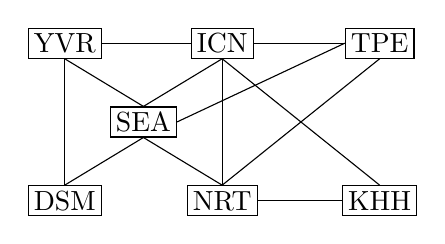
\begin{tikzpicture}
\node [rectangle] (YVR) at (-1,1) {YVR};
\node [rectangle] (DSM) at (-1,-1) {DSM};
\node [rectangle] (SEA) at (0,0) {SEA};
\node [rectangle] (ICN) at (1,1) {ICN};
\node [rectangle] (NRT) at (1,-1) {NRT};
\node [rectangle] (TPE) at (3,1) {TPE};
\node [rectangle] (KHH) at (3,-1) {KHH};

\draw (YVR.south) -- (SEA.north);
\draw (SEA.south) -- (NRT.north);
\draw (NRT.east) -- (KHH.west);
\draw (KHH.north) -- (ICN.south);
\draw (ICN.south) -- (NRT.north);
\draw (NRT.north) -- (TPE.south);
\draw (TPE.west) -- (ICN.east);
\draw (ICN.south) -- (SEA.north);
\draw (SEA.south) -- (DSM.north);
\draw (DSM.north) -- (YVR.south);
\draw (TPE.west) -- (SEA.east);
\draw (YVR.east) -- (ICN.west);
\end{tikzpicture}


%%%%%%%%%%%%%%%%%%%%%%%%%%%%%%%%%%%%%%%%%%%%%%%%%%
\verb|twoptwo|

\tikzsetnextfilename{twoptwo}
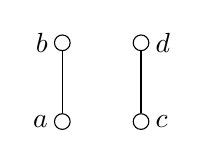
\begin{tikzpicture}
\node[label={left:$a$}] (a) at (0,0) {};
\node[label={left:$b$}] (b) at (0,1) {};
\node[label={right:$c$}] (c) at (1,0) {};
\node[label={right:$d$}] (d) at (1,1) {};

\draw (a) -- (b);
\draw (c) -- (d);
\end{tikzpicture}


%%%%%%%%%%%%%%%%%%%%%%%%%%%%%%%%%%%%%%%%%%%%%%%%%%
\verb|labeledpetersen|

\tikzsetnextfilename{labeledpetersen}
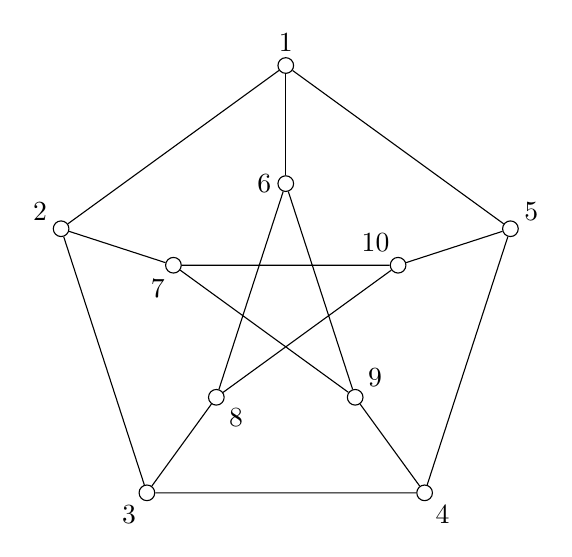
\begin{tikzpicture}
\foreach \i in {1,...,5} {
\pgfmathsetmacro{\ang}{18 + \i*72}
\pgfmathsetmacro{\pang}{108 + \i*72}
\pgfmathsetmacro{\j}{int(\i + 5)}

\node[label={\ang:$\i$}] (\i) at (\ang:3) {};
\node[label={\pang:$\j$}] (\j) at (\ang:1.5) {};
\draw (\i) -- (\j);
}
\draw (1) -- (2) -- (3) -- (4) -- (5) -- (1);
\draw (6) -- (8) -- (10) -- (7) -- (9) -- (6);

\end{tikzpicture}

\end{document}


%%% compile by pdflatex --shell-escape filename.tex
%%% then run ./pdf2png.sh *.pdf in figures/
